%Toy Falsification example
%\todo[inline]{skipping for now}
We can also formulate a falsification problem (\cite{AbbasATVA11_LinFalsification}, \cite{Deshmukh15_IterativeApproaches}) by minimizing robustness in order to find trajectories of a closed loop system that violate a specification. In particular, we solve the following problem:

\begin{subequations}
\vspace{-10pt}
\label{eq:falsification}
\begin{align}
\text{min}&_{x_0 \in X_0 } \, \srob_{\formula}(\sstraj) \nonumber \\
\text{s.t. } & x_{k+1} = f_k(x_0) \, \forall k=0,\dotsc,N-1 \\
&  x_{k} \in X \, \forall k=1,\dotsc,N
\end{align}
\end{subequations}

For evaluation, we solve the problem for the point-mass system of \eqref{eq:PointMass}, with a state feedback controller for fixed-point tracking to the state $[2.25,2.25]'$, which lies in the middle of the Terminal set (Fig. \ref{fig:toy falisification}). The specification is $\formula=\always_{[0,20]} \neg (x_k \in \text{Unsafe})$, where the set $\text{Unsafe}$ is as defined earlier. The set of possible initial state, $X_0$ is shown in Fig. \ref{fig:toy falisification}, as is the initial point (used for initialization in the optimizer) and resulting trajectory, which satisfies $\formula$ with a robustness of $1.25$. As before, $N=21$ is the length of the resulting trajectory under consideration.

For evaluation, we compare A) SQP using smooth robustness (SOP), B) gradient descent on robustness using SQP (R-SQP) and C) Simulated Annealing (SA) \cite{SA_book}. Initial states and trajectories from the 3 methods are shown in Fig.\ref{fig:toy falisification}. SOP and R-SQP result in an initial state of $x_0=[-2.3418\, -2.3418]'$, while SA gives $x_0=[-2.3371\, -2.3354]'$. The robustness for trajectories from both SQP based methods is $-0.99998$, while via SA is $-0.9968$. Note, the trajectories via either method are very close, and pass near the center of the $\text{Unsafe}$ set (the origin), where the robustness reaches its minima of $-1$. Also worth noting, that for the trajectory via method SOP, $\srob_{\formula}=-0.9932$, i.e. a relative approximation error of less than $1\%$ with respect to $\rob_{\formula}$.

\begin{figure}[t]
\centering
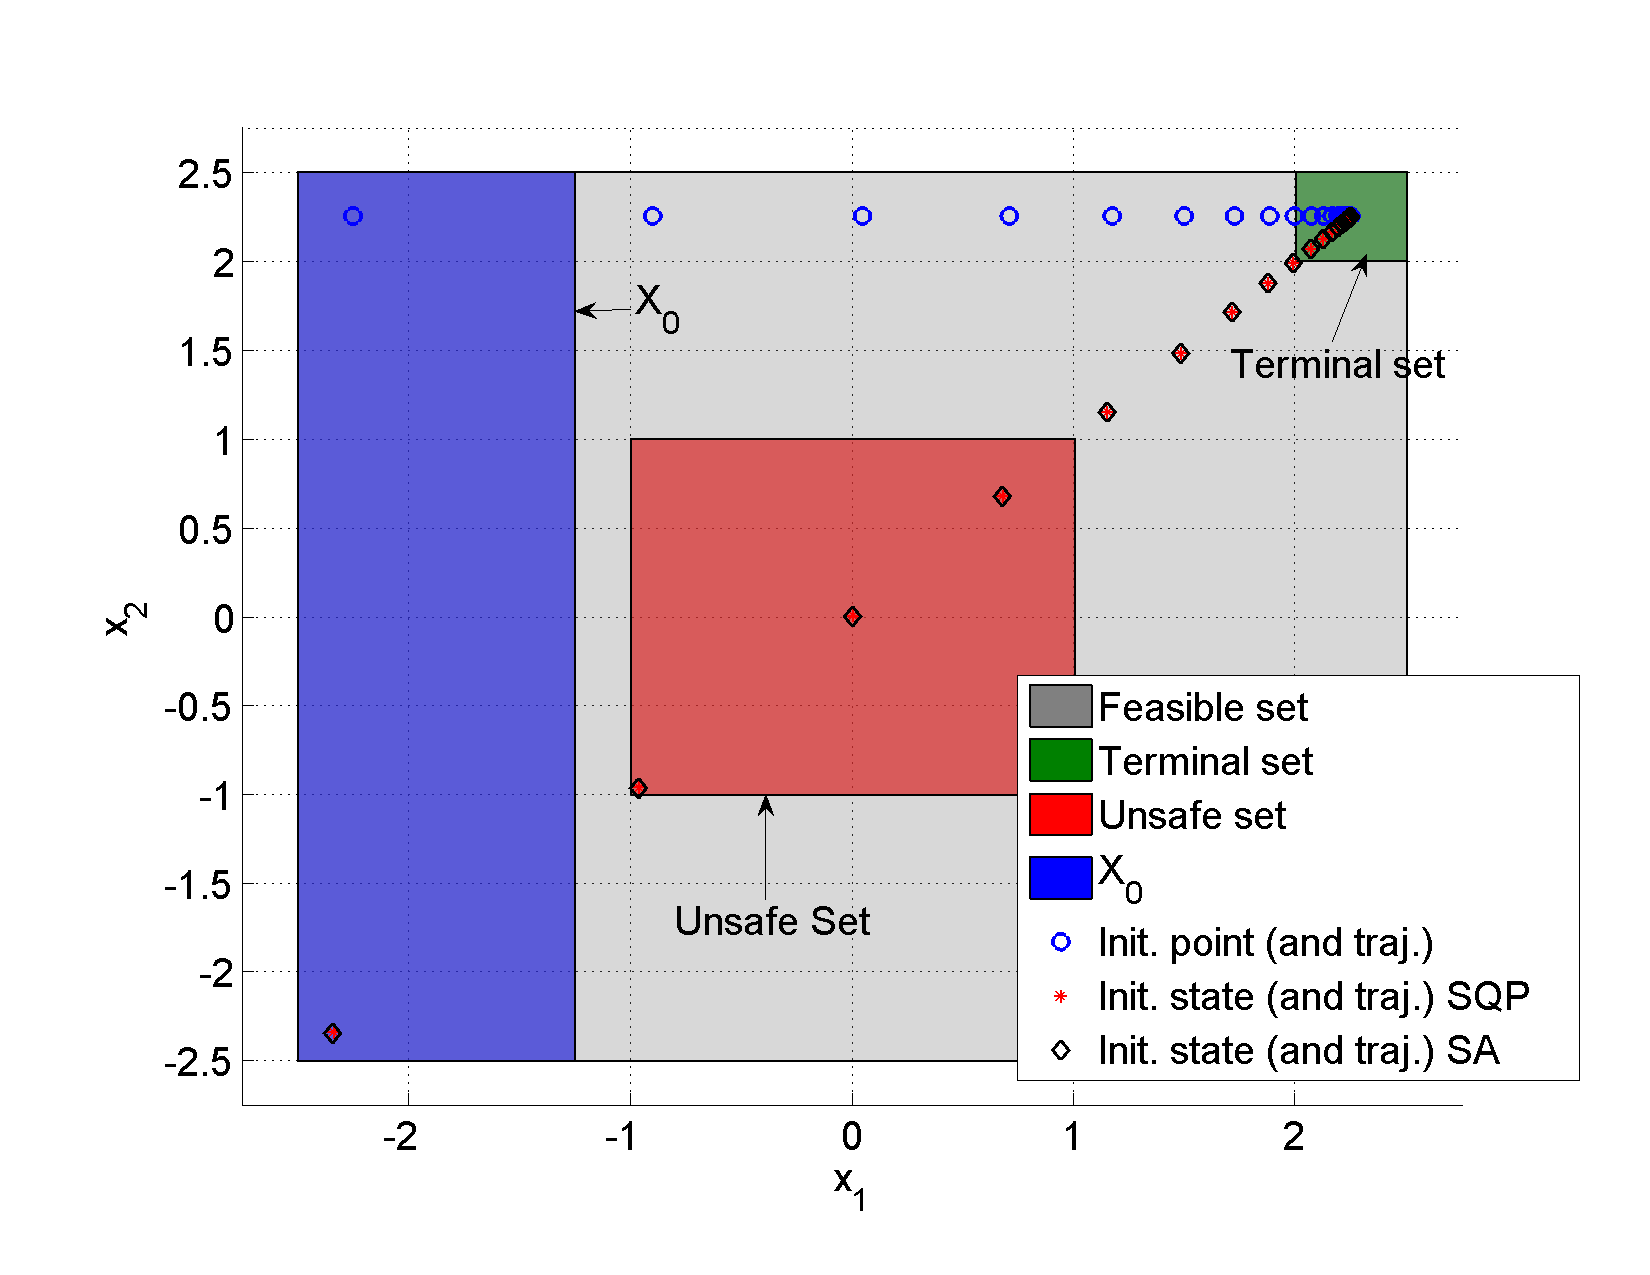
\includegraphics[width=0.49\textwidth]{figures/ToyExampleFalse}
\vspace{-30pt}
\caption{{\small Trajectories from initial points obtained from robustness minimization via SA and SOP, R-SQP (both of which lead to the same optimal solution)}}.
\label{fig:toy falisification}
\vspace{-20pt}
\end{figure}